\section{Discussion}
This Section will discuss the findings from the interview study. For hindering factors that were found, a possible solution will be discussed. For motivational factors, ways to further improve these factors will be taken into consideration.

\subsection{Motivational factors}
During the coding process of the interviews, several factors that motivated participants to use the prototype were found. Here, these motivational factors that were found during testing are discussed. Possible ways to further strengthen these points in future developments of the tool are proposed in this Section.

\subsubsection*{Easily understandable visualizations}
The participants said that the visualizations were easily understandable. Future development should keep in mind that the ability to quickly understand the visualizations motivated the participants to discuss the results further, rather than being preoccupied trying to understand what the visualization tries to show them.

To keep the visualizations easily readable, the paradigm \emph{one job per visualization} should be followed. The clear separation of concerns between the two visualizations seemed to support the participants when answering questions. If new visualizations should be added to the tool, this should be done in a separate chart, rather than by adding new elements to one of the existing charts.

The separation of the visualizations could be deepened even further by showing the different visualizations in different tabs. During the user tests, the participants rarely referred to the other visualization during interpretation.

\subsubsection*{Interesting results}
Participants said that the results are interesting and surprising, which according to \citeauthor{northMeasuringVisualizationInsight2006} is an indicator that they could gain insight. Future versions of the prototype could allow participants the easy exporting of specific results to share them with interested friends if they find results surprising or interesting. Participants also reported that the tool made them reflect their own beliefs of how social networks work and how discussions unfold.

\subsubsection*{Supporting explanatory texts}
The explanatory texts helped the participants understand the visualizations and the capabilities of the tool better. As discussed in chapter \ref{sec:missingExamples}, these explanatory texts can be further improved, e.g., by adding examples and hints for analysis.

One thing that could be changed about the explanatory texts is their position. Due to the nature of Observable, which was used to build the prototype, explanatory texts were always visible and did not only show in context. One way to further improve the way the texts are presented is by visually hiding some of the texts in the interface. For this, texts should be divided into two kinds:
\begin{enumerate}
    \item Texts that are essential to understanding the visualizations
    \item Texts that offer additional help, insights, explanations, or inspiration for analyzing the data set
\end{enumerate}

Dividing texts into these two categories could result in a less cluttered interface. Important texts from the first category can always be shown, while texts that fall into the second category can be hidden, e.g., in tooltips or detail panes. Showing only necessary texts also means that the visualizations are front-and-center in the tool, attracting the users' attention. It would also eliminate the need to scroll a lot when accessing the tool from a laptop or tablet (cf. m26, l. 75). One example of how these hints could be shown can be seen in figure \ref{fig:sentiment_tooltip_hint}.

\begin{figure}[htb]
    \centering
    \fbox{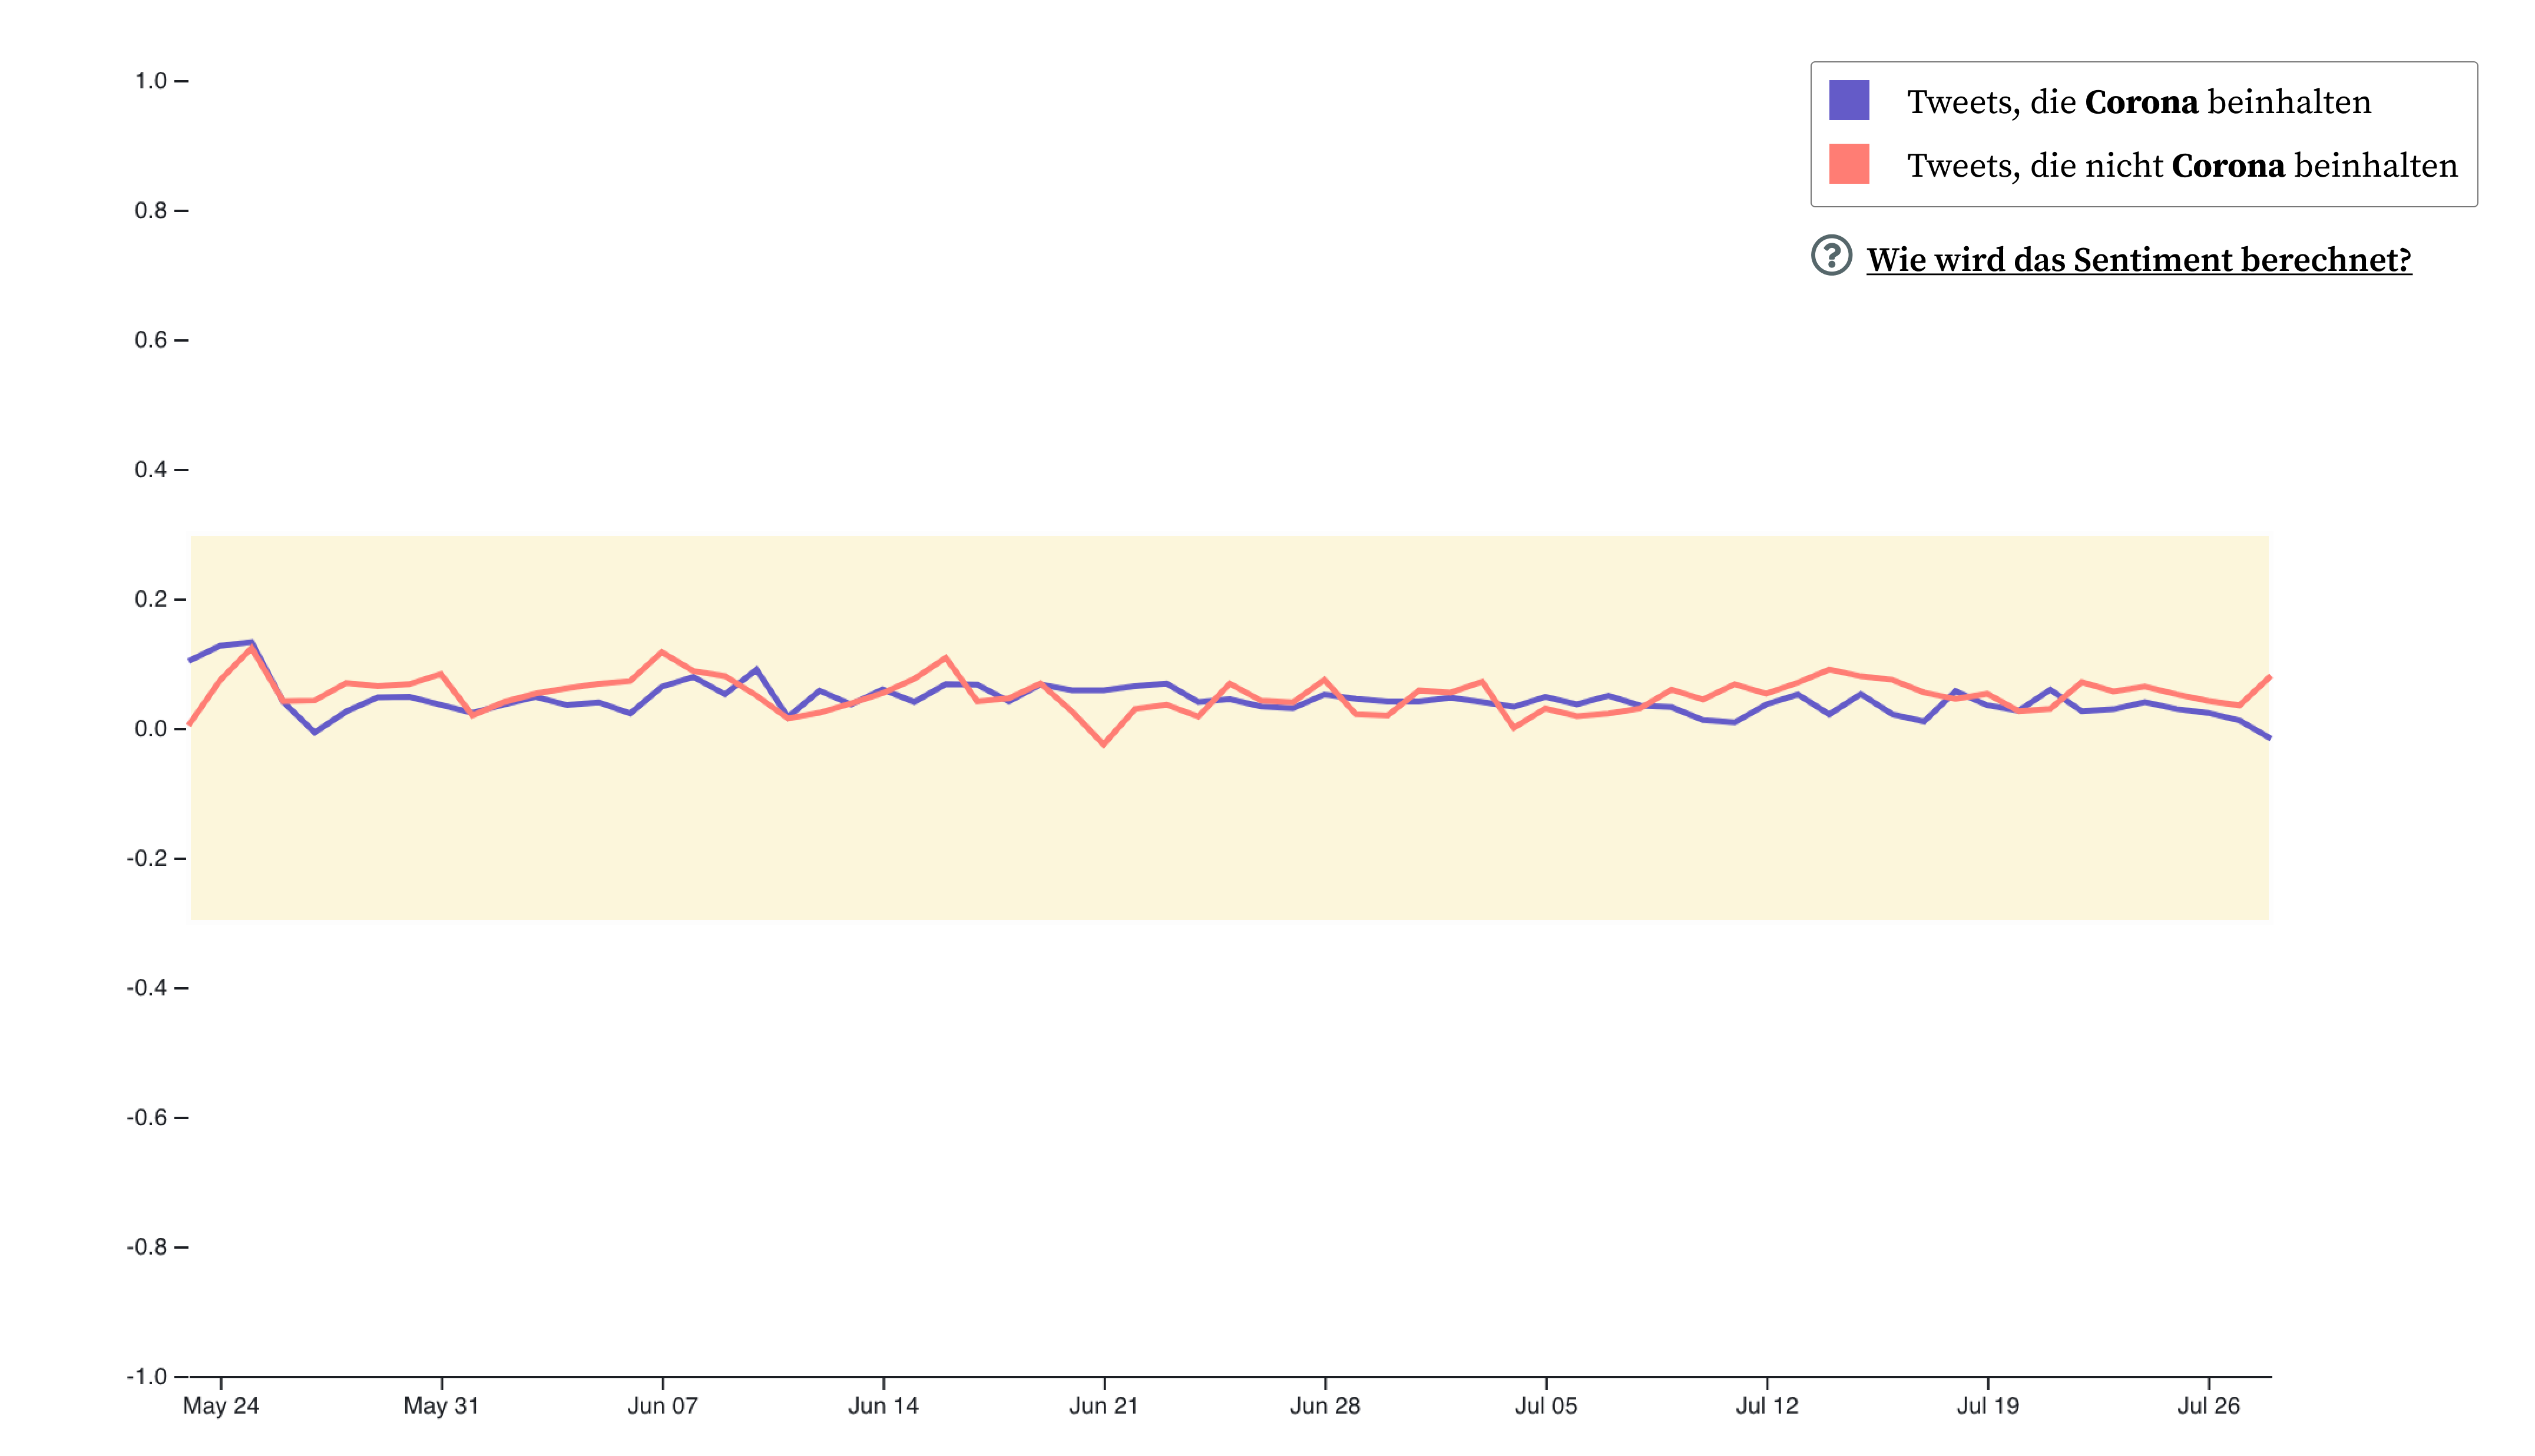
\includegraphics[width=0.98\linewidth]{images/sentiment_tooltip_hint.png}}
    \caption{A proposed tooltip target for additional explanations regarding the sentiment analysis.}
    \label{fig:sentiment_tooltip_hint}
\end{figure}

\subsubsection*{Filters can be applied quickly}
Except for the word filter, which had to fetch new data from the database, the filters could be applied quickly. This seemed to support how participants worked with the tool while solving the tasks during the interview as well as during the free exploration. This suggests that future development should focus on keeping the interaction with these filters quick.

During user tests, the toggles were mostly used for a before-and-after view of the dataset, e.g., quickly toggling the retweets to visually compare the impact the retweets had on the tweet volume. This interaction could be further improved. One example could be to introduce a button that can be held down to turn all filters on or off. Holding down the button could show the 'original' data set without the retweet- or neutral tweet filters applied, letting go of the button shows the filters the users applied before again. A similar interaction can be found in image manipulation software like Apple Photos, where holding a button switches between the original photo and the manipulated version.

\subsubsection*{Tooltip with further information}
The tooltip that was shown in the volume chart helped participants finding answers to their questions. Future development could focus on making this tooltip more helpful. One important step for this would be to create a more visually appealing tooltip which contains styled information. The tooltip that was eventually used in this study could only handle single strings of unstyled text. However, text styling is one of the most efficient ways to structure information so that it can be easily digested. 

\subsection{Hindering factors: Missing interface components}
Some of the problems that were mentioned can be solved by introducing additional interface components. The problems and their proposed solutions are discussed in this Section.

\subsubsection*{Overview of currently set filters}
Multiple participants had trouble recognizing what data filters were applied for the current visualization. The idea that the filters can be changed on top of the notebook and will then influence the rest of the visualization does not seem to work, especially on smaller laptops, as this resulted in a lot of scrolling.

\begin{figure}[htbp]
    \fbox{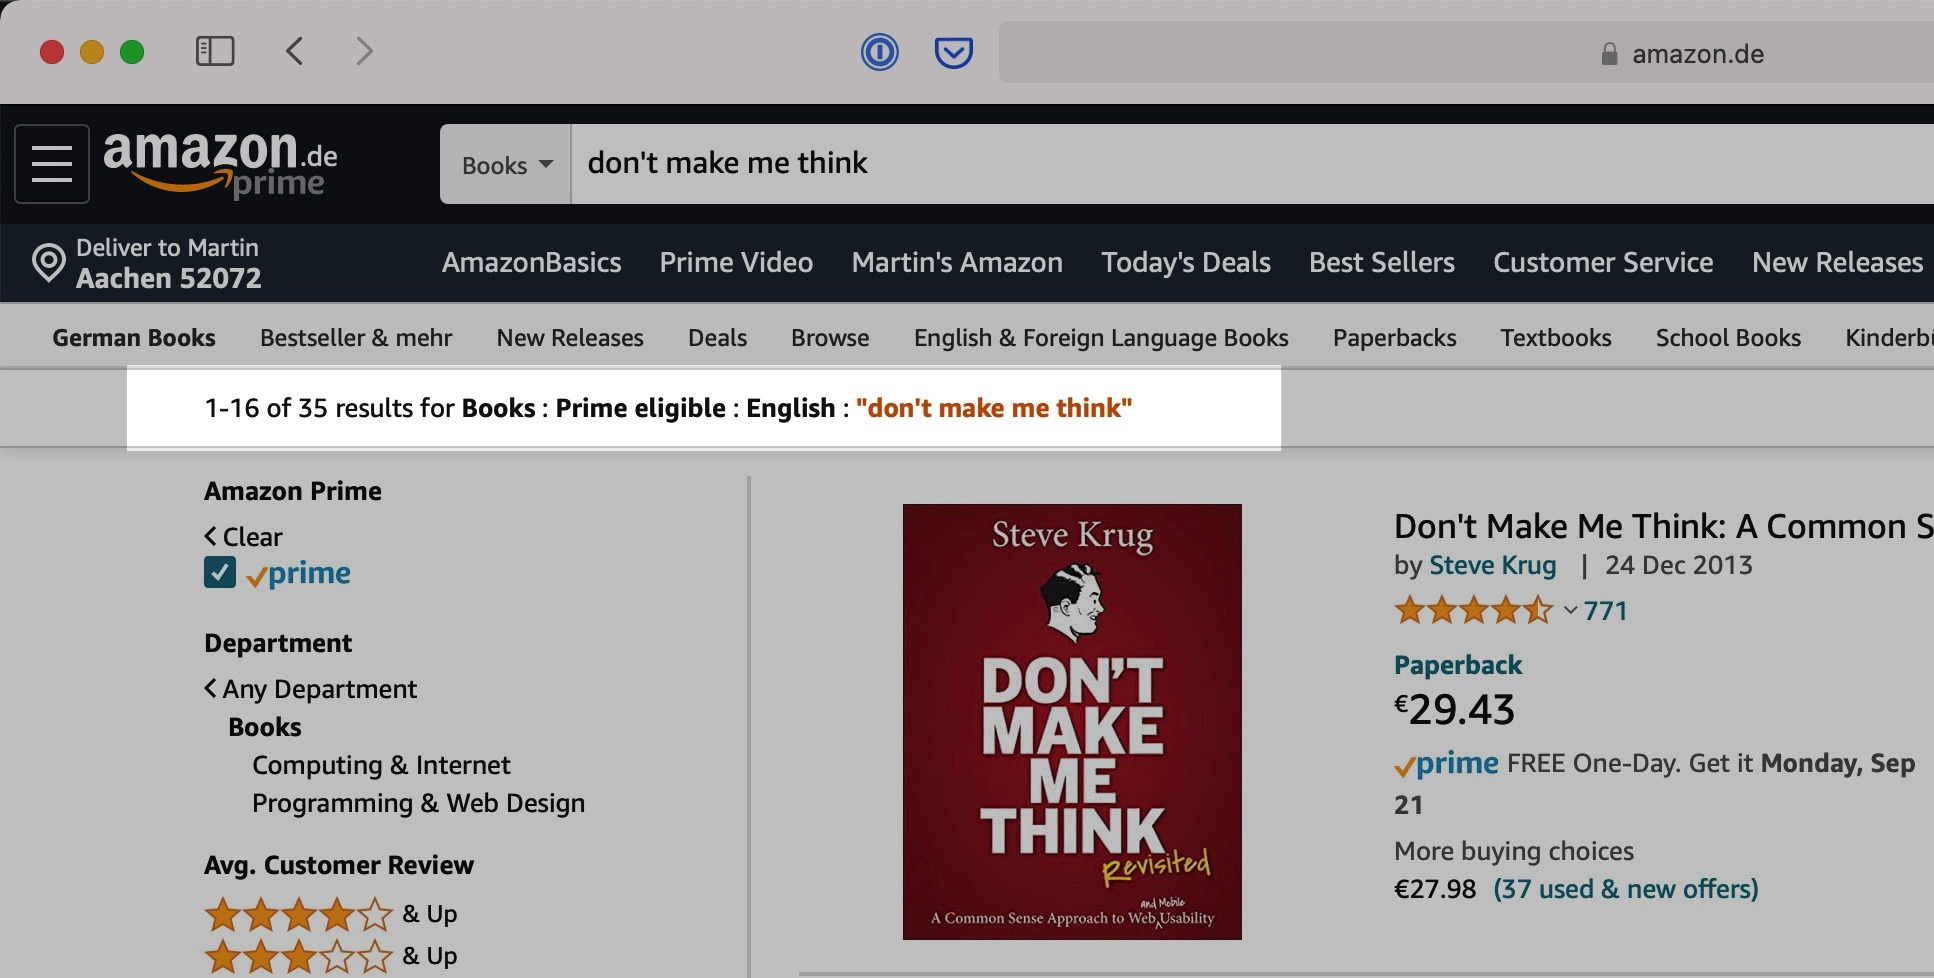
\includegraphics[width=\linewidth]{images/amazon_filters.jpg}}
    \caption{The Amazon search is filtered to English-language books which are eligible for prime-shipping, with the search input \emph{don't make me think}. Highlight by the author.}
    \label{fig:amazon_filters}
\end{figure}

This means that the filter status should be visible directly next to the visualization. This way, participants would not need to search for the current filter status. Rather, the status would almost always be in view while interpreting the visualizations. There are two possible ways to show the filters near the visualizations:
\begin{enumerate}
    \item \textbf{Show a descriptive text above the visualization:} Using a text to show the status of the filter could help participants to quickly understand what kind of data the visualization is showing at the moment. One example of this technique can be found on Amazon, as seen in \textbf{Figure \ref{fig:amazon_filters}}. This technique is especially useful when a lot of different filters can be applied.
    \item \textbf{Show the filter toggles right next to the visualization:} Instead of showing the filter status as a text, showing the filters with the actual toggles would allow users to change the filters right next to the visualization. A mock-up for this solution can be seen in \textbf{Figure \ref{fig:legend_and_filters}}.
\end{enumerate}

\begin{figure}[h!tb]
    \fbox{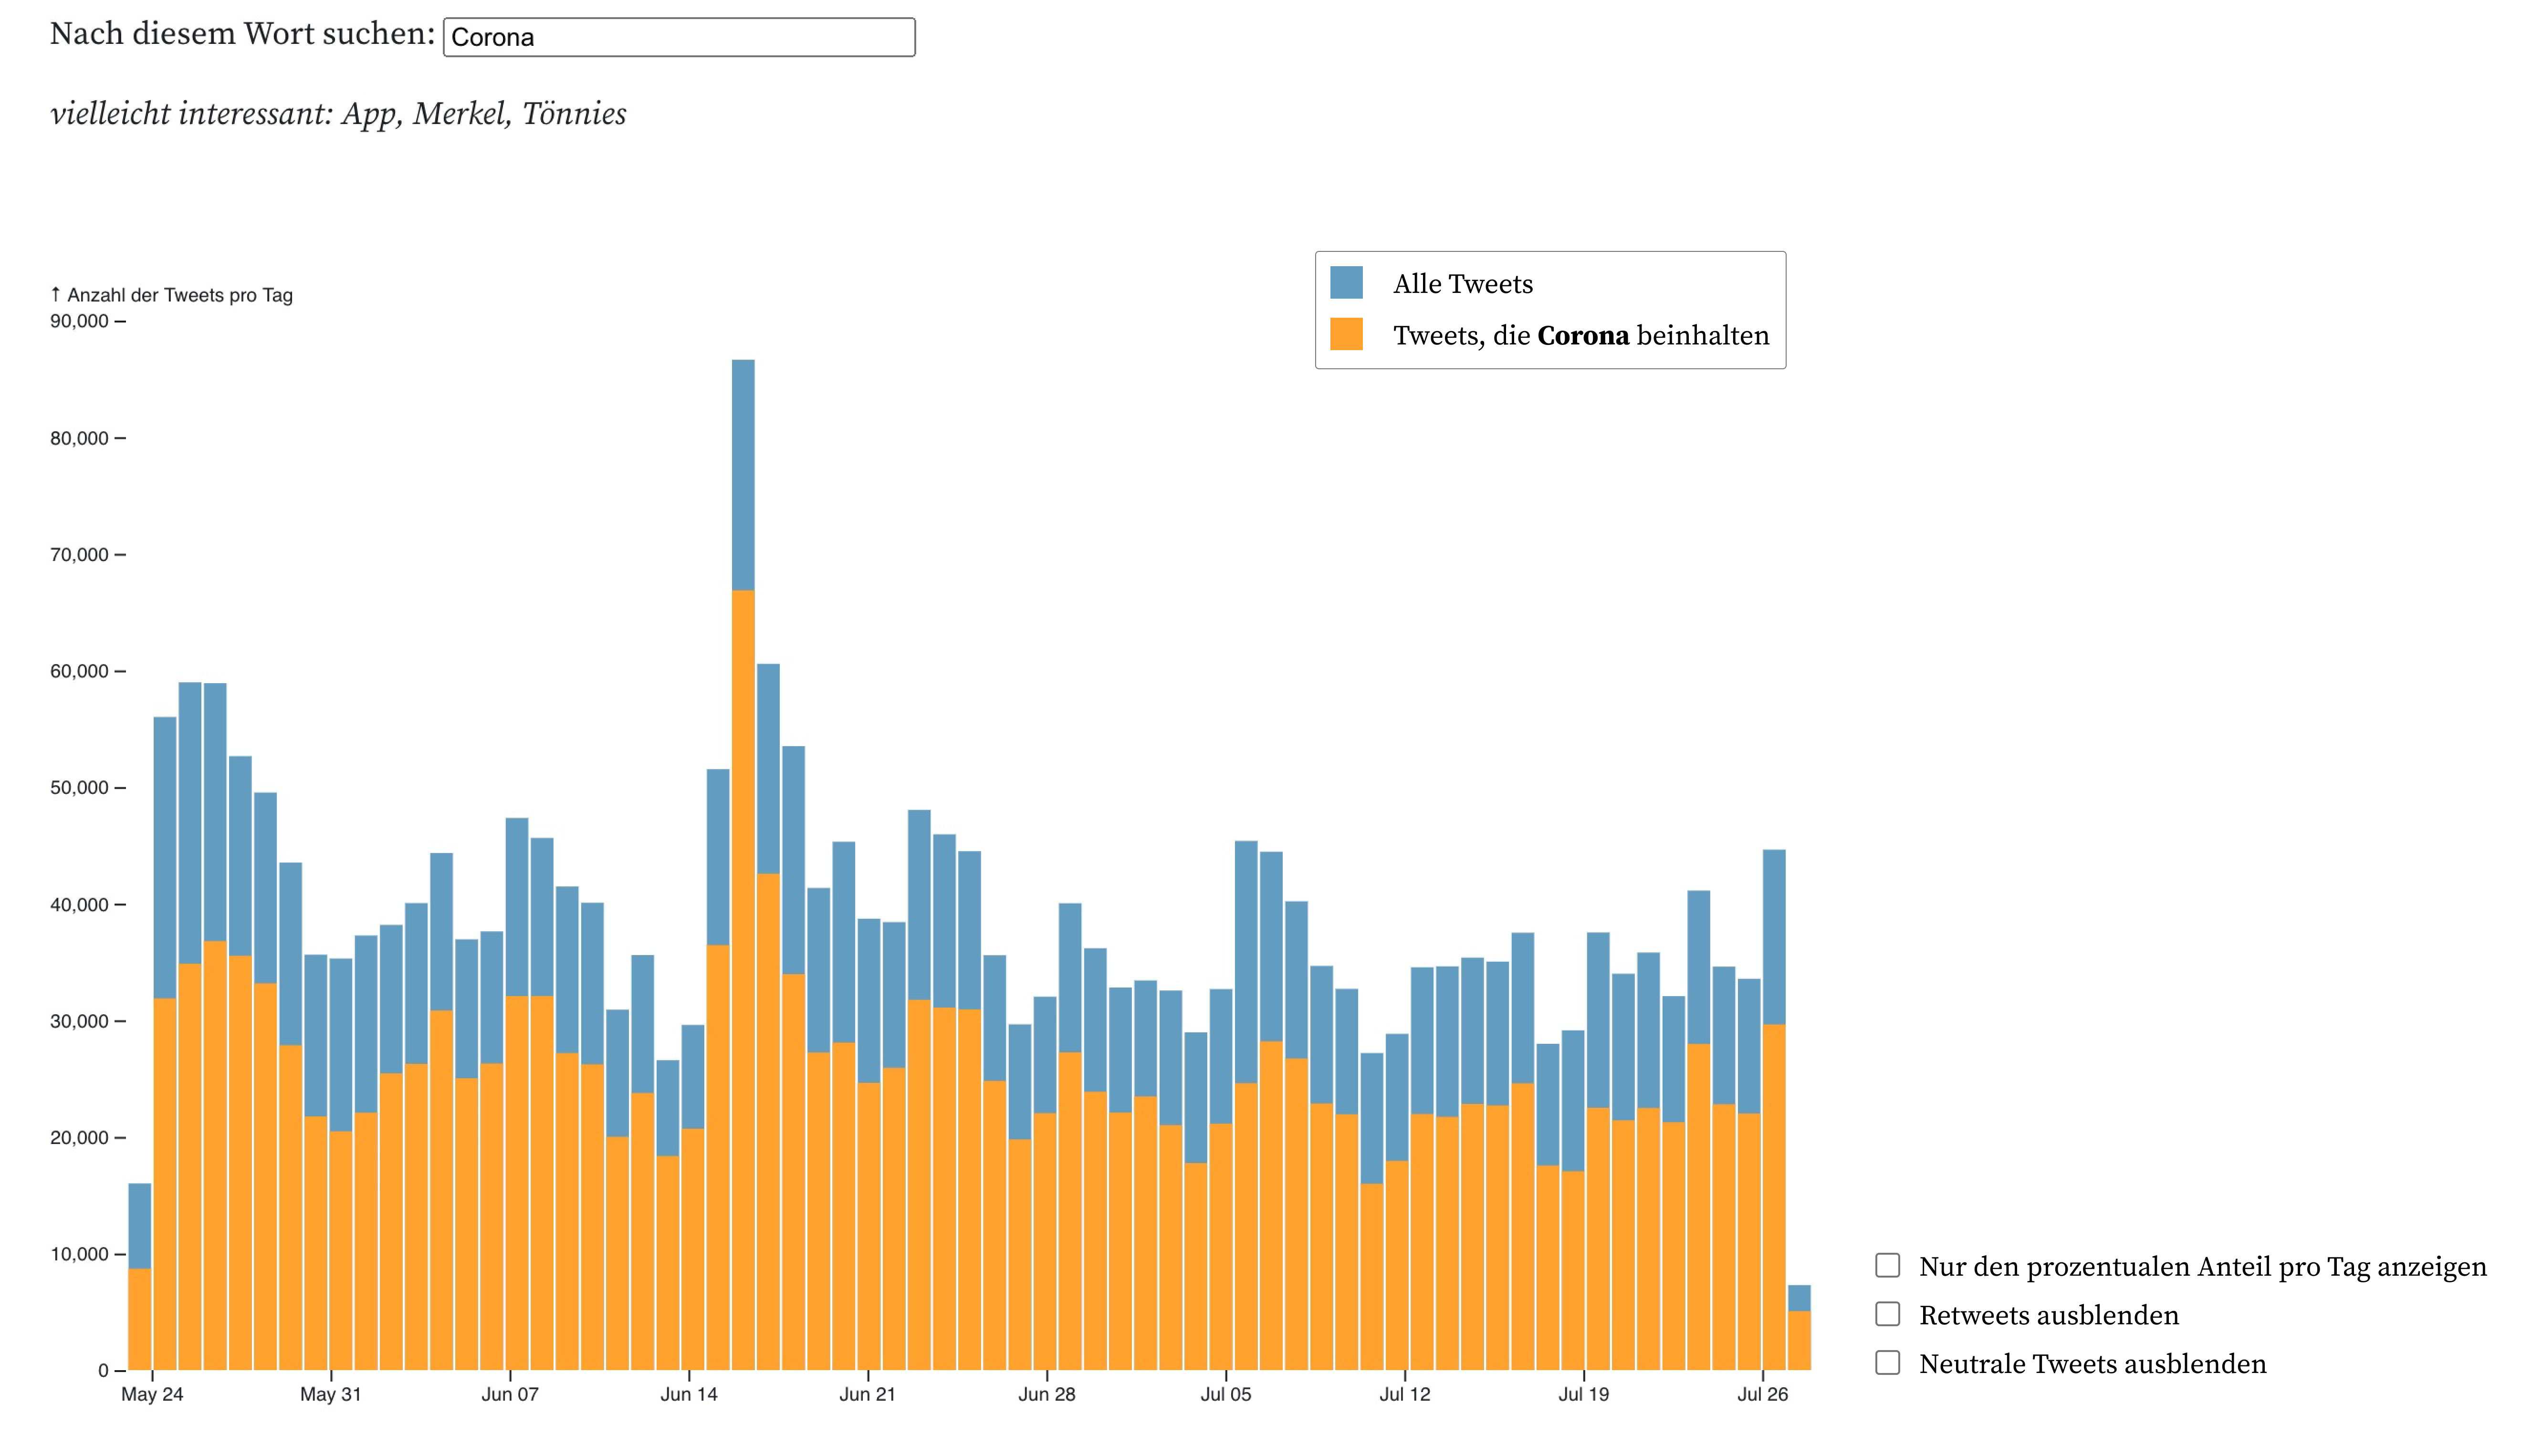
\includegraphics[width=\linewidth]{images/legend_and_filters.png}}
    \caption{Proposed layout of the tweet volume with a legend and filters directly next to the graph.}
    \label{fig:legend_and_filters}
\end{figure}

Showing the filter toggles right next to the visualizations seems like a straightforward idea. However, this raises the question if the filters of the two visualizations should be linked or not, i.e., should the filter of the sentiment graph change as well when the filter of the volume graph is changed or not? To decide this, further studies should be conducted to see if the synchronicity of the data visualizations is helpful or not.

This study did not examine if it helps users to have a single filter context within several visualizations or not. During the exploration phase in the interview, however, the participants did not seem to switch a lot between examining the tweet volume and the sentiment chart. This could suggest that having a single filter applied to both visualizations is not a necessity. In this case, using two independent filter sets that are independent of each other could avoid user confusion as only explicit user actions influence the visualization.

\subsubsection*{Color legend}
Another missing interface component are colored legends. During user testing, several problems arose because of the missing legend. For one, the graphs were less self-contained. Users were forced to read the explanatory texts that accompanied the graphs to be able to understand what the different colors mean. Another problem with the textual explanation of colors was that different participants would have named the colors differently than the text did and were confused, e.g., when the text talked about a light-red line, but the participants only identified an orange one. A legend like the one shown in \textbf{Figure \ref{fig:legend_example}} could have helped to identify the colors more easily, as well as making the graph more self-explanatory.

\textbf{Figure \ref{fig:legend_and_filters}} shows a proposed addition to the tweet volume-graph. Implementing these changes makes the current filter status more obvious and lets users toggle the different filters without needing to scroll to the top of the notebook again. The legend with dynamic labeling, which includes the search term the user entered, makes the graph more self-contained.

The added legend could also help solve the layout problem that participants mentioned. With the explanatory texts no longer necessary to understand the graphs, the texts serve as an additional explanation and, as such, can remain below the graph itself.

\subsubsection*{Loading indicator}
Another component that was missing from the interface was an indicator that new data was fetched from the server. One possibility to show this fetching would be to show a small loading indicator next to the word filter. However, this position may not be noticeable enough. It would also not indicate that the visualization does not yet reflect the selected data set.

Another possibility would be to show in the visualizations themselves that new data is being fetched. As fetching takes about 5 seconds and the visualizations have not been updated before the fetching is complete, it should not be a big problem to visually hide the visualizations during the fetching stage. A possible solution for this can be seen in \textbf{Figure \ref{fig:fetching_state}}.

\begin{figure}[htb]
    \fbox{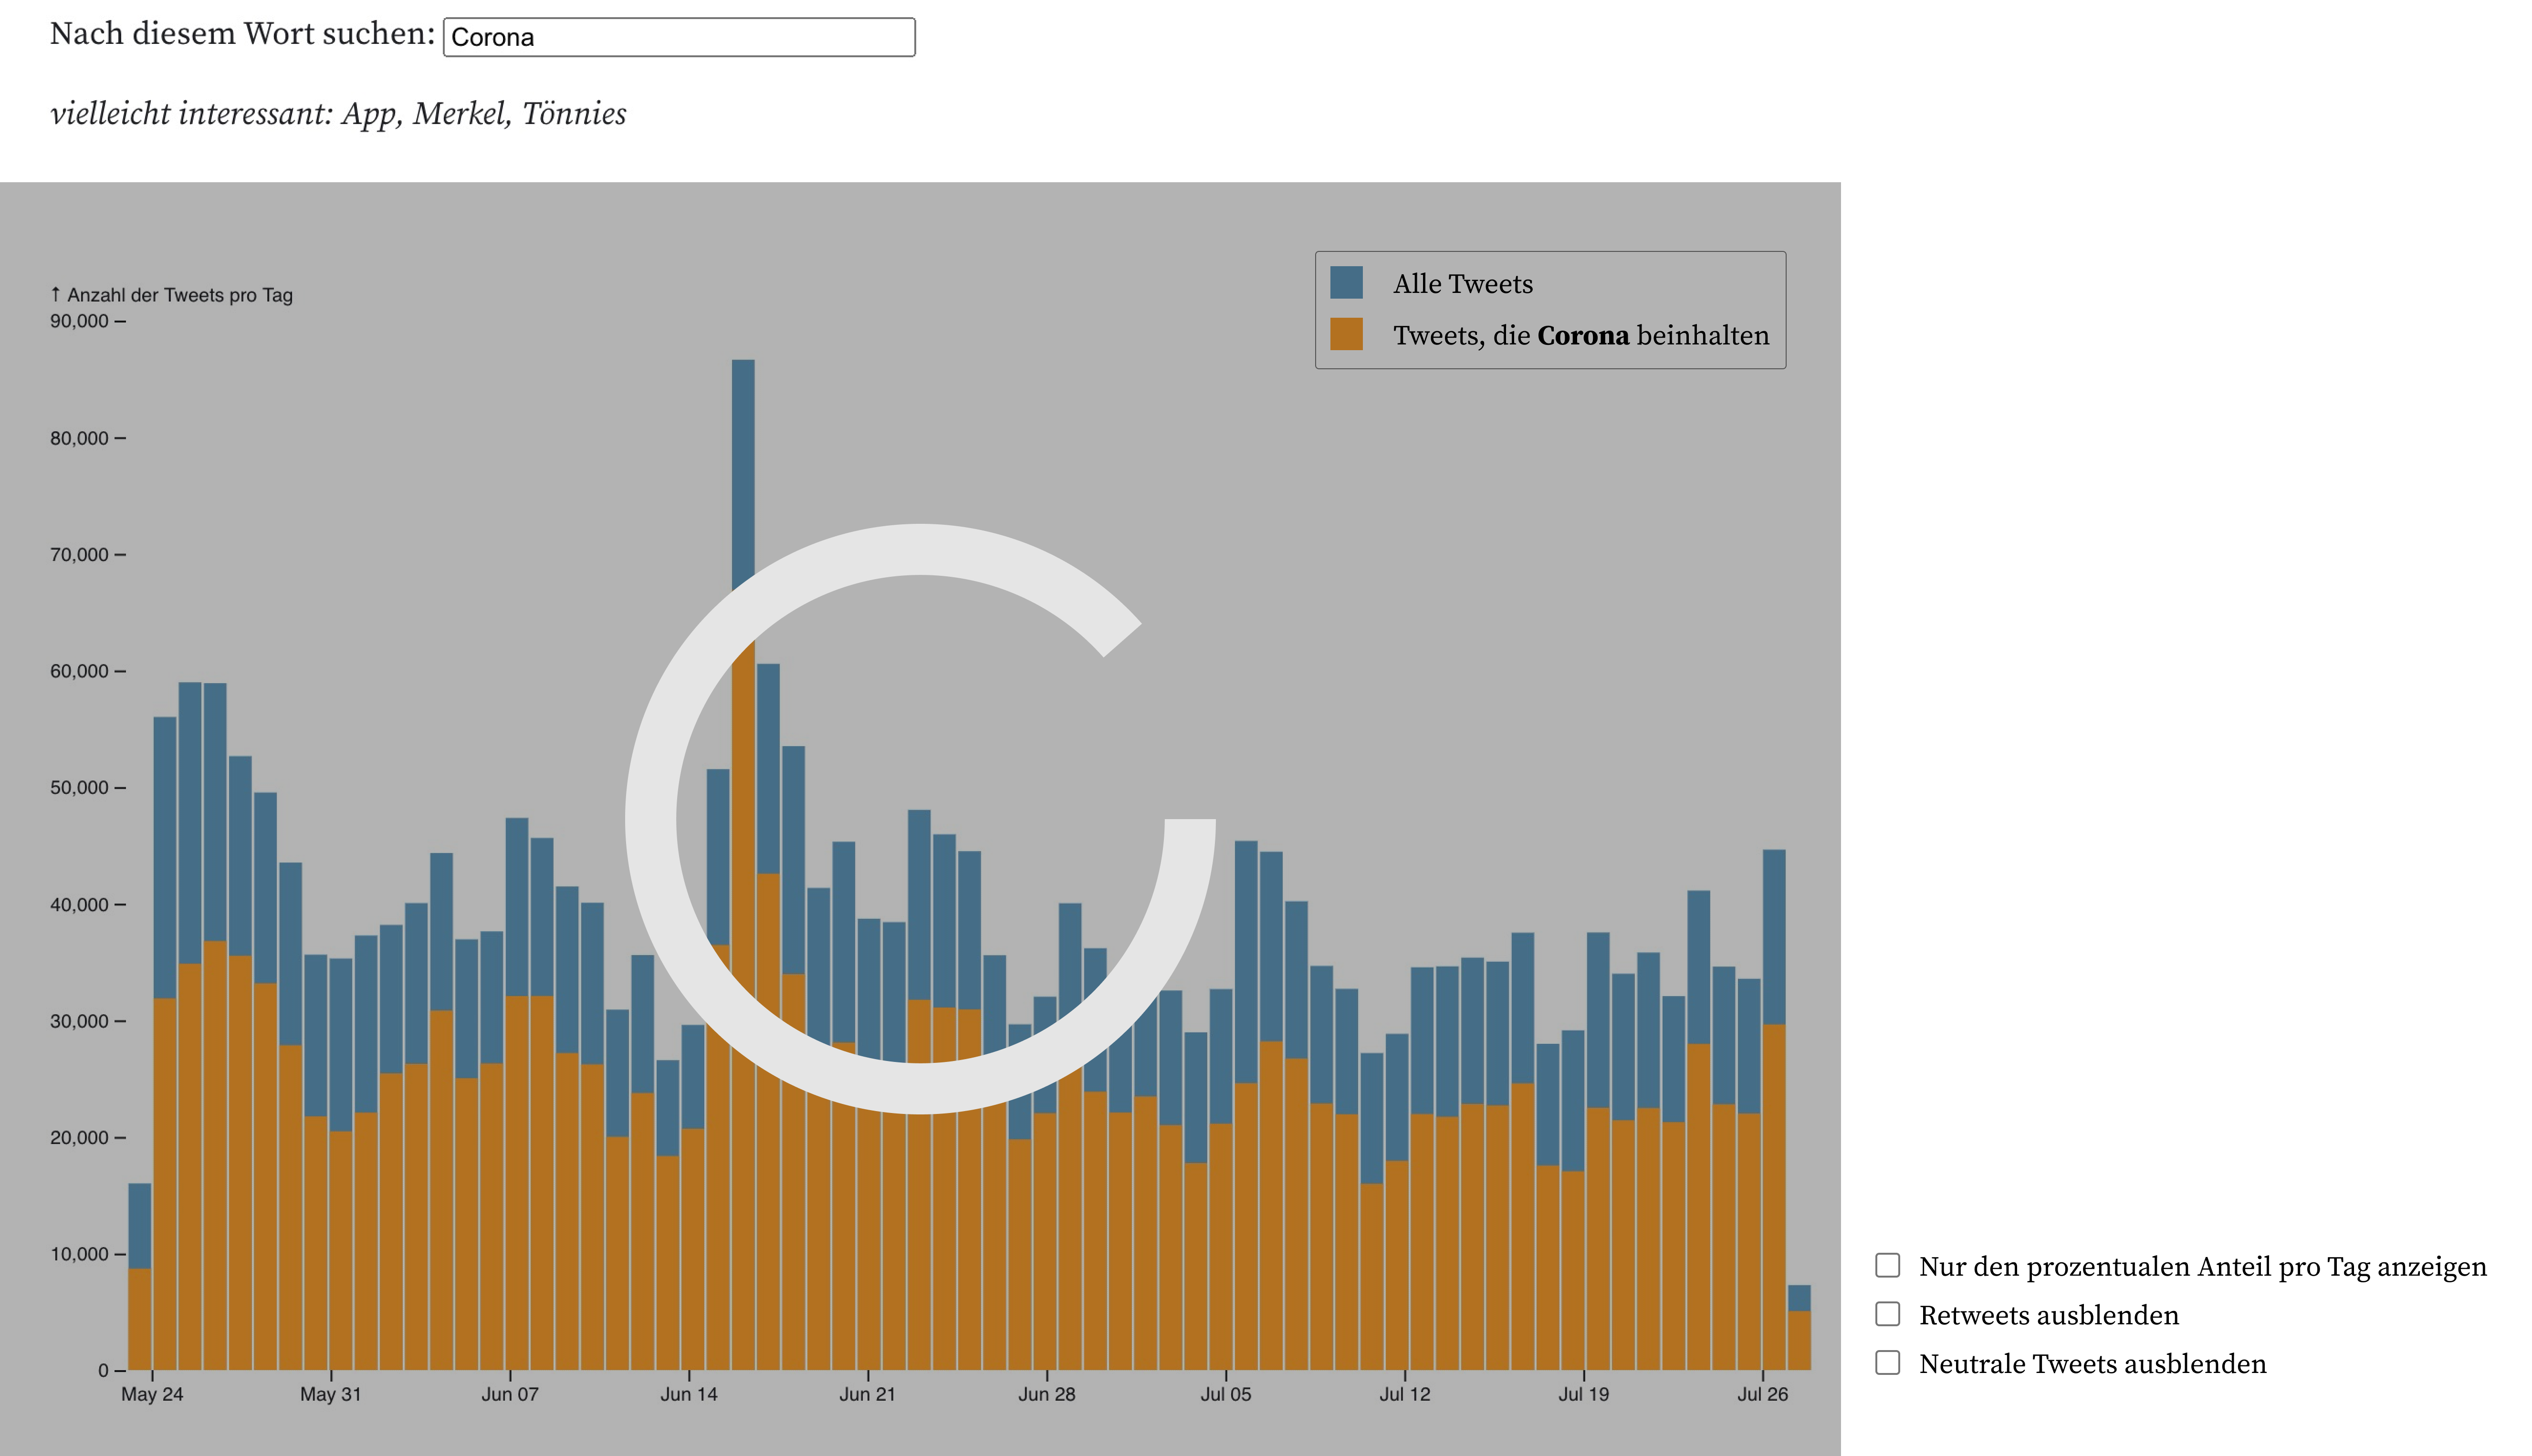
\includegraphics[width=\linewidth]{images/fetching_state.png}}
    \caption{Proposed solution to show that new data is being retrieved from the server.}
    \label{fig:fetching_state}
\end{figure}

\subsection{Hindering factors: Missing information}
The contents of this Section are about pieces of information that participants said they would expect to be able to interpret the data more efficiently. This information can be textual or visual: Textual information means written text, some additional explanation of how to work with the tool, or more detailed information. Visual information means, e.g., more emphasis on certain aspects of the charts, or highlighted information.

\subsubsection*{Missing real-world context}
One idea that was not implemented due to time constraints was to give participants some context as to what happened on specific days based on the tweet-texts themselves. Because the calculated collocations did not yield satisfying results, this feature was not implemented for the prototype of the dashboard. This cut feature is further discussed in Section \ref{sec:cutForTime}.

Some participants explicitly said that they would have liked to know what happened on specific days, especially when they recognized spikes in Twitter activity for a topic or spikes in the sentiment on a specific day. Further development of the tool should take this into account and, e.g., collect daily Twitter trends using the Trend API\footnote{https://developer.twitter.com/en/docs/twitter-api/v1/trends/trends-for-location/api-reference/get-trends-place, last visited on Sep. 24, 2020 \\}. This would allow participants to analyze the dataset more thoroughly. In several interviews, participants said that they would have wanted more context to understand spikes in the tweet volume or the sentiment graph. They expected this information to be present in the prototype itself, and no participant searched the internet for further information on what happened on these days.

The Twitter trends could give at least some hints on what might have happened on these days. These trends, or trending topics, are names, phrases, or topics that are mentioned significantly more often than others. Those trending topics are fleeting, however. A study examining the trends on Twitter found that most of the trends stayed in the top 10 or even top 50 of the trending topics for less than an hour (\cite{annamoradnejadComprehensiveAnalysisTwitter2019}). This makes it necessary to aggregate the trends per day.

Showing participants the trending topics for specific days could also solve another problem that became visible during the user tests. During the free exploration in the interviews, some participants immediately had ideas that they wanted to check in the dataset (see, for example, w26b, l. 9: \say{Ich probier es mal mit Stuttgart denn da gab es ja glaub ich eine der ersten dieser Hygiene-Demos}). Others only explored the data set that was open when the notebook was first opened. This dataset showed the complete dataset, including retweets and neutral tweets, with the word filter \emph{Corona} applied. Showing daily trends could give participants ideas on how to explore the data set further.

\subsubsection*{Missing examples for the sentiment graph}\label{sec:missingExamples}
Some participants said that they found the sentiment analysis interesting. Some wished for further explanation on how the sentiment is computed and also wished to see examples of tweets with a sentiment of +1 and a sentiment of -1 (see m23, l. 73: \say{Also klar, was das irgendwie bedeuten soll, aber... wie sieht jetzt zum Beispiel ein positiver Tweet aus oder ein negativer.}).

\begin{figure}[htb!]
    \centering
    \fbox{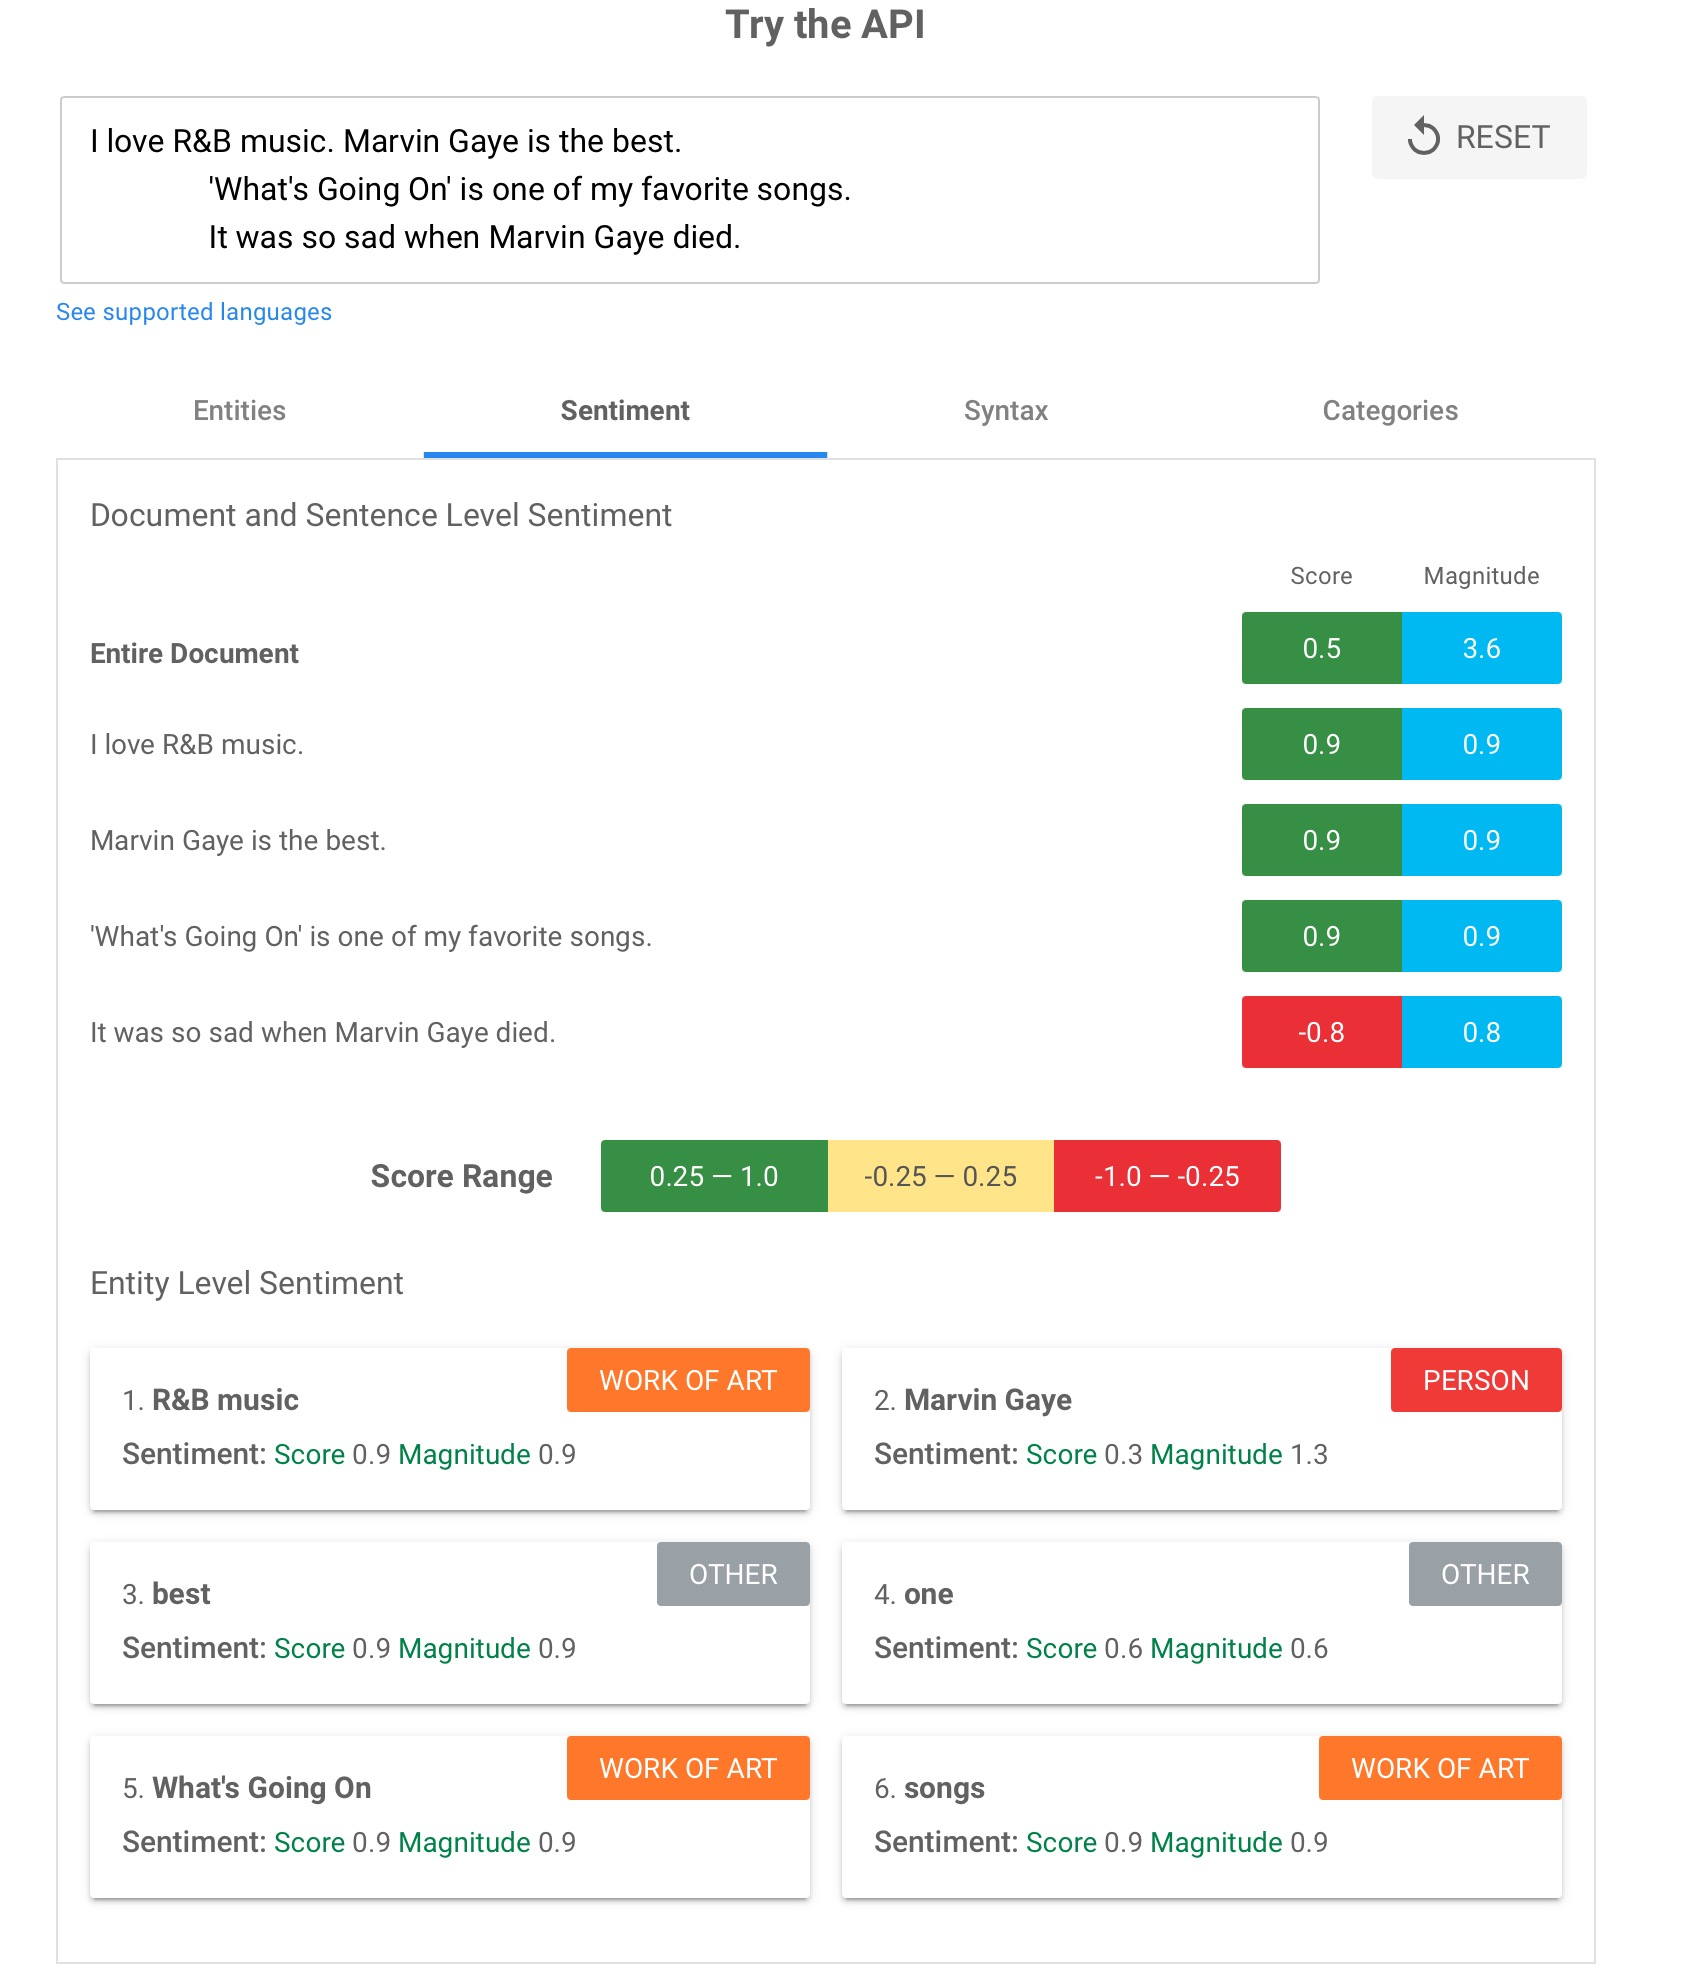
\includegraphics[width=0.8\linewidth]{images/sentiment_google.jpg}}
    \caption{The demo shows the sentiment of the full text, of the complete sentences, and for individual entities in the text.}
    \label{fig:sentiment_google}
\end{figure}

The same participant also said that he would have liked some advice on how to correctly interpret the sentiments, as well as potential pitfalls for the analysis that he should take care of. This explanation could be done in a similar way as Google explains the sentiment analysis in their Natural Language API Demo\footnote{https://cloud.google.com/natural-language/natural-language-api-demo, last visited on Sep. 24, 2020\\}, as seen in \textbf{Figure \ref{fig:sentiment_google}}. According to the participants, they would not want such an explanation for every single tweet, but rather for selected examples. This means that these examples could be hard-coded in the interface and would not have to be dynamically generated from the dataset.

At the same time, other participants said that a lengthy explanation on how the algorithm works would not have helped them and that they preferred not to have additional explanations. This means that an explanation should be an optional interface component, e.g., a tooltip near the sentiment graph. This allows interested users to access the information, while users who do not want to learn more about sentiment analysis can focus on interpreting the data at hand.

\subsubsection*{Neutral tweets-area was not marked as such}
When asked to interpret the sentiment graph, multiple participants focused on the threshold of ±0.3 for neutral tweets. This threshold was mentioned for the explanation of the \emph{neutral tweets}-toggle and is, as discussed in chapter 2, a common threshold to differentiate between neutral tweets and tweets that carry an opinion. The participants looked for peaks above or below ±0.3 to find days where the discourse on Twitter was especially emotional. This could be facilitated by marking this area in the chart itself, similar to how the 0-baseline was marked. An example for this can be seen in \textbf{Figure \ref{fig:sentiment_neutral_area}}.

\begin{figure}[h!tb]
    \centering
    \fbox{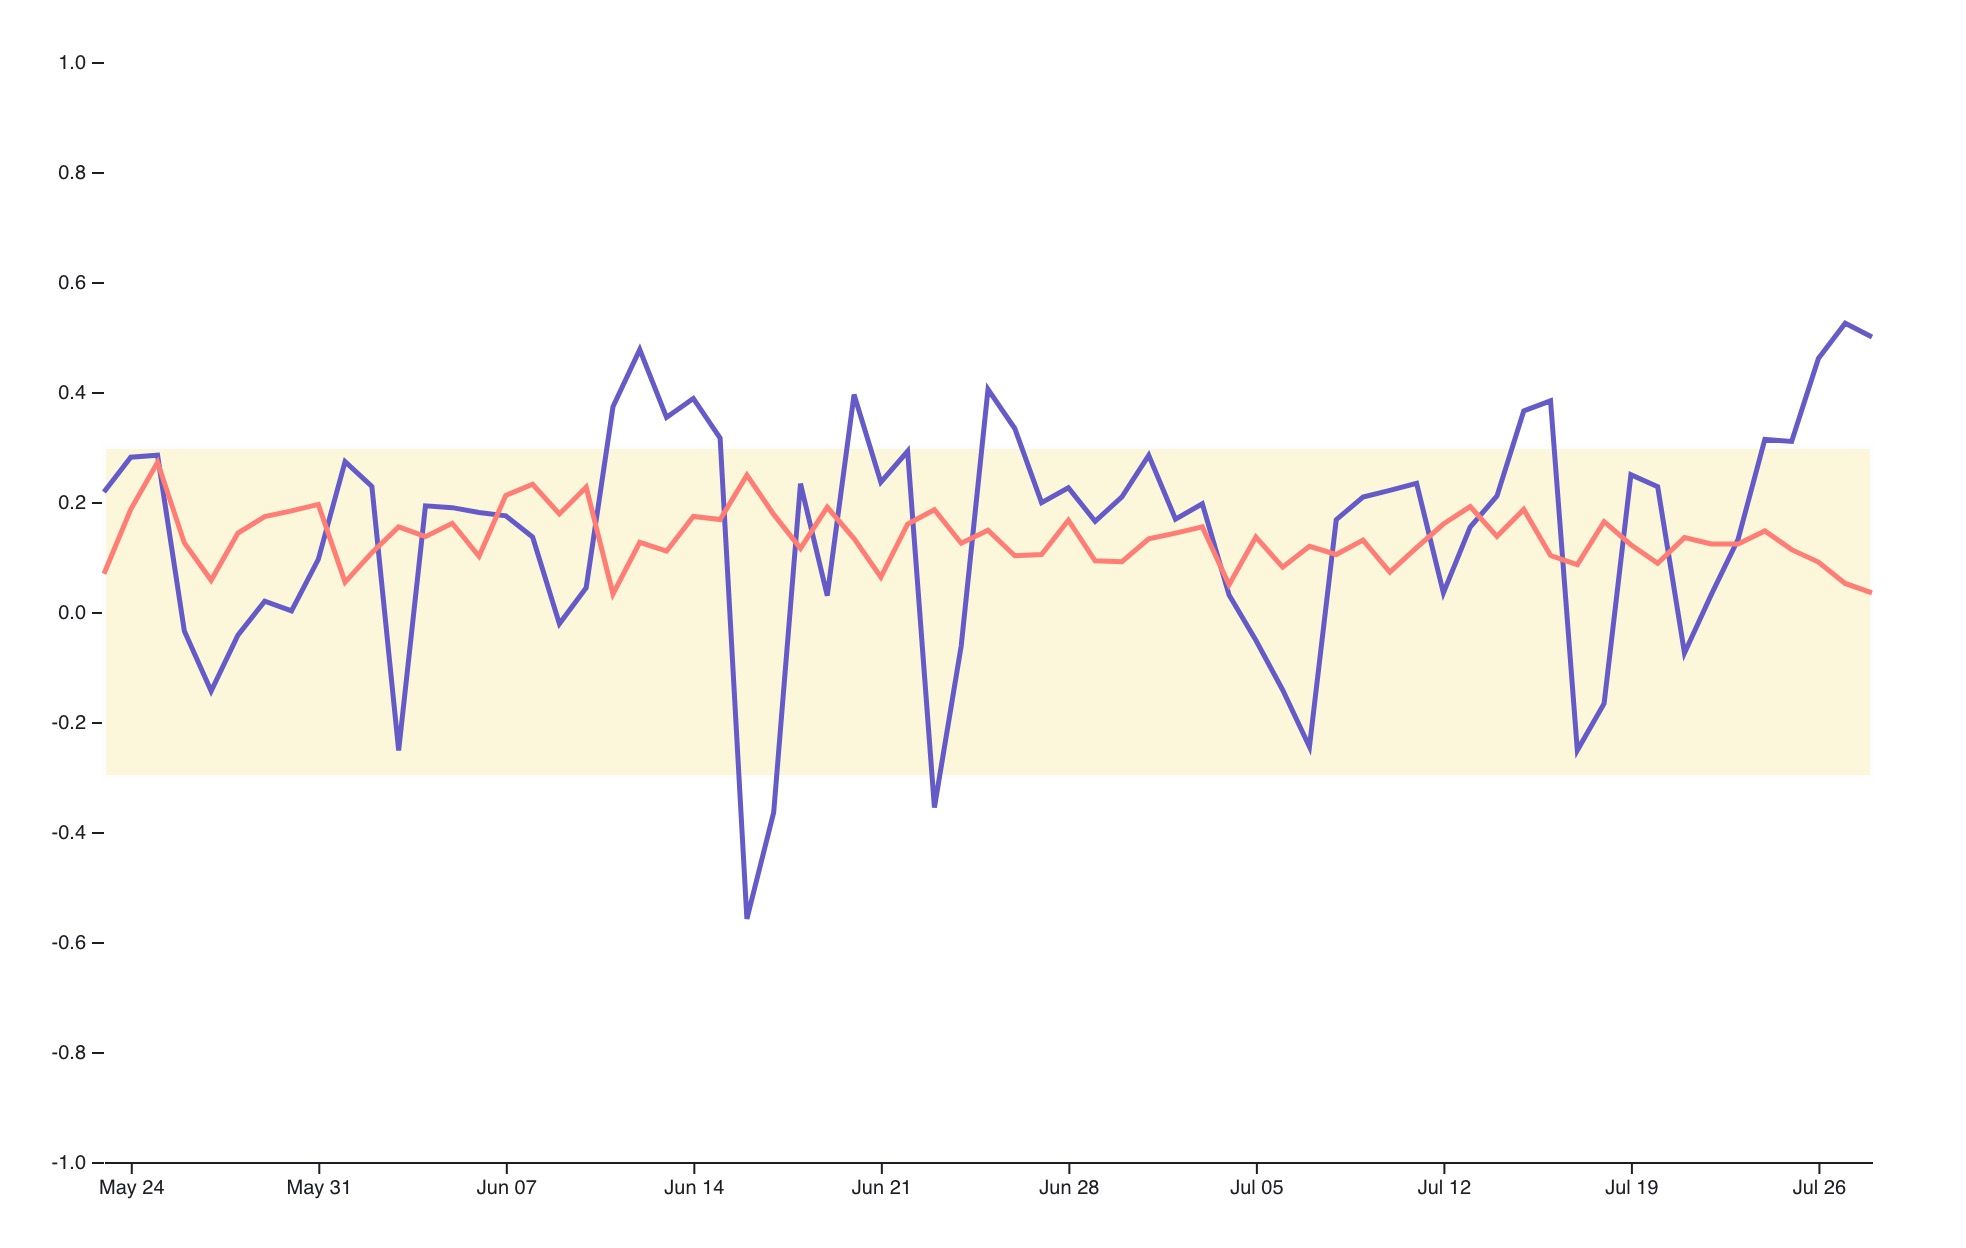
\includegraphics[width=0.98\linewidth]{images/sentiment_neutral_area.jpg}}
    \caption{The area containing the neutral tweets is marked, making it easier to identify spikes above or below the threshold. The screenshot shows the data when filtered for \emph{Drosten}.}
    \label{fig:sentiment_neutral_area}
\end{figure}

\subsection{Hindering factors: Technical limitations}
This Section discusses findings from the interview where technical limitations hindered participants from solving tasks. Some of these limitations were conscious trade-offs for this prototype version. Nonetheless, these issues should be addressed if a tool based on this prototype should be further developed.

\subsubsection*{Fixed data set} \label{sec:fixedDataSet}
The fixed data set came up in one interview where the participant tried to scroll the data set to reveal even more days. This revealed one of the biggest disadvantages of using Twitter's streaming API to collect tweets in real-time (see Section \ref{sec:fetchedData}). Using this method guarantees the most complete data set on the free tier of Twitter's API, at least from the time the data collection is started. The downside is that using this API makes it impossible to access past tweets. Users of the tool have to recognize a potentially interesting topic very early, start the data collection, and then wait some time until enough data has been gathered.

Using the paid API to access Twitter's archives could solve this problem, at least in parts. The paid access to Twitter's archives gives access to the past 30 days of activity on Twitter, which could give a 'headstart' to the data collection. For a final version of this tool, a combined approach could be possible: using the real-time data collection of a specific topic with the streaming API, and simultaneously fetching the last 30 days of Twitter activity to this topic. This would mean that users would be able to analyze the past month of tweets directly from the beginning of the data collection, eliminating the need to wait some days before they can gather meaningful results from Twitter.

If this approach would be used, the data collection pipeline would have to be modified further. In the current implementation, the sentiment of a tweet is computed synchronously when the tweet is sent to the collecting app by the streaming API. The data sent by the Twitter archive may be too big to compute the sentiment synchronously. In this case, users should get a message that the sentiment is being computed, but that they can already start analyzing the volume graph.

Allowing users to explore a bigger data set could mean that the way the data set is presented has to be changed. One example of showing a data set that spans multiple months can be seen on Spiegel Online (\cite{merlotCoronavirusBrasilienManaus2020}, see also the screenshot \textbf{Figure \ref{fig:spiegel_visualization}}).

\begin{figure}[htb!]
    \fbox{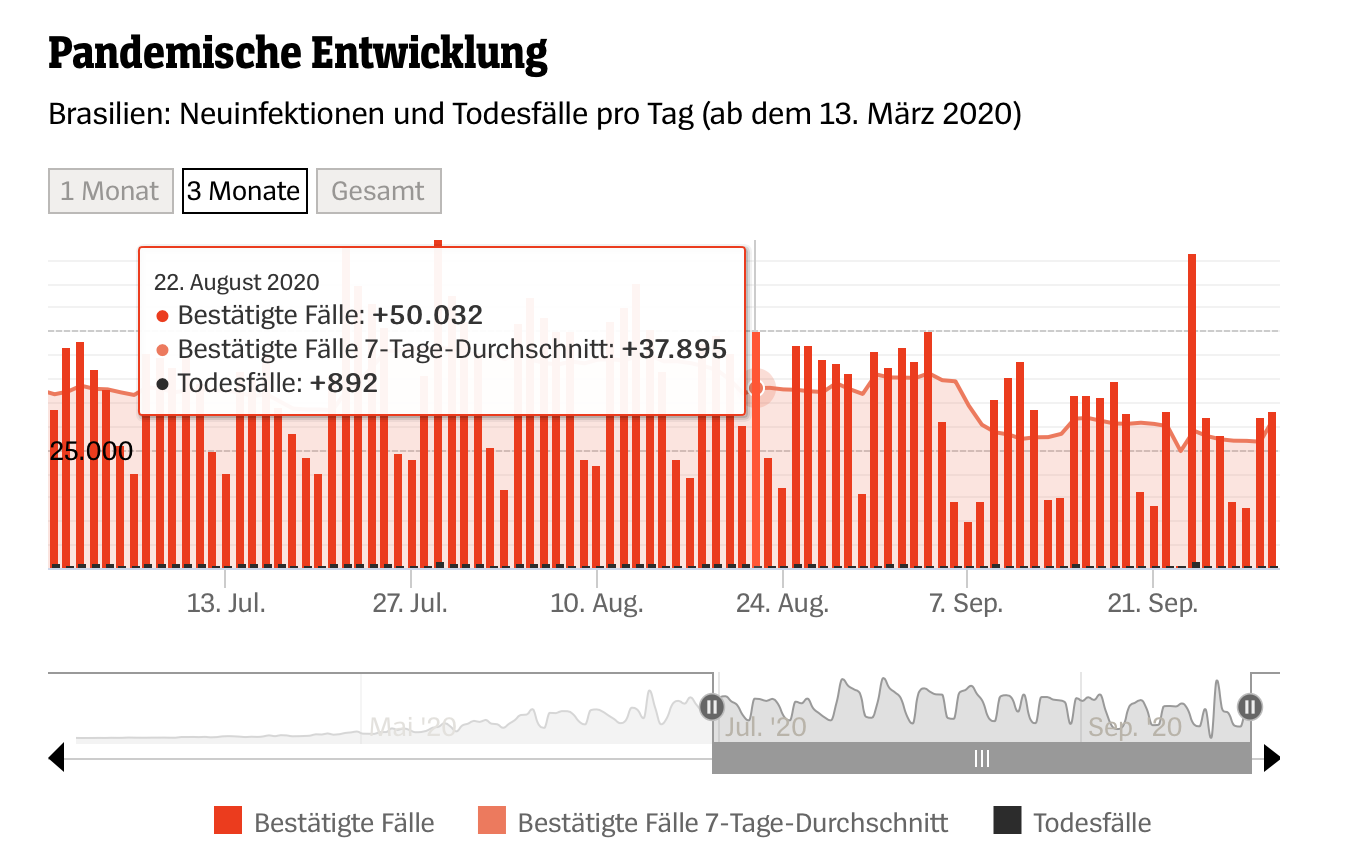
\includegraphics[width=\linewidth]{images/spiegel_visualization.png}}
    \caption{A coronavirus visualization from Spiegel Online. The buttons on top select the time frame that should be displayed. The scroll bar below the chart allows users to move the viewport to explore other parts of the dataset. Users can also drag the size of the scroll bar to change the time frame that is displayed. Taken from \cite{merlotCoronavirusBrasilienManaus2020}.}
    \label{fig:spiegel_visualization}
\end{figure}

The chart showing the new infections and Corona-related casualties in Brazil can be manipulated by users in different ways:
\begin{itemize}
    \item Buttons on top of the chart let users switch the scope of the data set between 1 month, 3 months, and the whole data set.
    \item The scroll bar allows users to move the selected time frame. This means they can see data from the last three months starting today, from the last three months starting next week, or wherever users move the scroll bar.
    \item The scroll bar can also be resized. By doing this, users can choose a time frame other than the default three options.
\end{itemize}

Similar to what was already mentioned in this discussion, the visualization from Spiegel Online also has a tooltip which shows more detailed information and a visual legend that explains the colors in the graph. 

\subsubsection*{Basic word filter}
Another problem that needs further technical work is how the word filter works. The current implementation acts as a case-insensitive filter that looks for parts of words. This means that, if a user enters \emph{App}, tweets containing these sorts of texts will be found:

\begin{itemize}
    \item I like this \textbf{App} a lot
    \item Whats\textbf{App} collects your data
    \item What kind of video \textbf{app} would you recommend?
    \item I'm not angry, just dis\textbf{app}ointed
\end{itemize}

This is different from how search engines, like DuckDuckGo, Google, or Bing, work. These engines use a so-called \emph{fuzzy search} which not only looks for the word itself, but also catches typographic mistakes, looks for synonyms, and so on.

Using a fuzzy search would allow users to explore the database more efficiently. During testing, for example, it was shown that typographic mistakes in the filter field would mean that little to no results were found, assuming that most of the Twitter users wrote the word correctly. The participant in question thought that there was not a lot of Twitter activity about the specific topic she was interested in. After one participant was told to correct the typo, she noticed an interesting pattern in the tweet activity and was able to interpret the data further. This means that it could be helpful to implement a fuzzy search to further develop the prototype.

\subsubsection*{Tooltips for the sentiment graph}
During the user tests, the participants expected to find tooltips for both graphs once they found the tooltip in the volume graph. This means that tooltips should either be used globally for all visualizations, at least where the additional information provided by the tooltip adds to the value. Alternatively, no tooltips at all could be used. As the tooltip in the volume graph helped participants to further explore the dataset, it should be kept for all the visualizations. Those tooltips would also satisfy \citeauthor{shneidermanEyesHaveIt1996}'s \emph{details-on-demand} by showing additional information when the user wants to see them, instead of cluttering the interface. Because of the way the tooltips were implemented in this prototype, they could not be added to the sentiment graph. More on this limitation can be found in Section \ref{fw_tooltips}.
